\documentclass[a4paper,fleqn]{article} %Options in documentclass should be set to a4paper and fleqn.
\usepackage{modsim}
\usepackage{times}
\usepackage{psfrag}
 \usepackage{pstricks}
 %\usepackage{auto-pst-pdf}
\usepackage{pstool}
\usepackage{natbib} %The three packages modsim, times and natbib are required.
\usepackage{amsmath, amssymb, amsthm} %Also recommend the standard AMS LaTeX maths packages.
\usepackage{changes}

\newcommand\solidrule[1][0.25cm]{\rule[0.5ex]{#1}{1pt}}
\newcommand\dashedrule{\mbox{%
		\solidrule[2mm]\hspace{2mm}\solidrule[2mm]}}
\pagestyle{MODSIMheadings} %Calling the MODSIM Headings format
\MODSIMhead{J. Pitt {\it et al.}, Dispersion and Shoaling Waves} %This is the content of the headings in all pages (except the first page). The format should be author, title of paper. If the title is too long, then use ... at the end. If more than two authors, then please use the "et al." format with et al. in italic, for example A. Author {\it et al.}, Title of the paper.

% Define any other command or required packages below:
%%%%%%%%%%%%%%%%%%%%%%%%%%%%%%%%%%%%%%%%%%%%%%%%%%%%%%%%%%%%%%%%%%%%%%%%%%%%%%%%%%%%%%%%%%%%%%%%%%%%%%%%%%%
\usepackage{rotating}
\usepackage{amsbsy,enumerate}
\usepackage{graphicx}
\usepackage{ccaption}
\newcommand{\ve}{\varepsilon}
\newcommand{\sigmah}{\hat{\sigma}}
\newcommand{\sigmab}{\bar{\sigma}}
\newcommand{\R}{\mathbb{R}}
\newcommand{\Z}{\mathbb{Z}}
\newcommand{\E}{\mathbb{E}}
\newcommand{\Tbar}{\bar{T}}
\newcommand{\Thetabf}{\mathbf{\Theta}}
\newcommand{\Xbf}{\mathbf{X}}
\newcommand{\xbf}{\mathbf{x}}
\newcommand{\Ybf}{\mathbf{Y}}
\newcommand{\ybf}{\mathbf{y}}
\newcommand{\Ubf}{\mathbf{U}}
\newcommand{\Fbf}{\mathbf{F}}
\newcommand{\fbf}{\mathbf{f}}
\newcommand{\Pbf}{\mathbf{P}}
\newcommand{\Pbfbar}{\bar{\mathbf{P}}}
\newcommand{\Sb}{\bar{S}^{\nu}}
\newcommand{\Snuib}{\tilde{S}^\nu _i}
\newcommand{\Snui}{S^\nu _i}
\newcommand{\sigmanui}{\sigma ^\nu_i}
\newtheorem{lemma}{Lemma}
\newtheorem{corollary}{Corollary}
\newtheorem{assumption}{Assumption}
\newtheorem{theorem}{Theorem}
\newtheorem{remark}{Remark}
\newtheorem{definition}{Definition}
\newtheorem{cce}{Assumption CCE}
\newtheorem{proposition}{Proposition}
%% The next four lines create the correct format for Figure and Table captions. They require the package "ccaption".
\makeatletter
\renewcommand{\fnum@figure}[1]{\textbf{\figurename~\thefigure}. }
\renewcommand{\fnum@table}[1]{\textbf{\tablename~\thetable}. }
\makeatother

\definechangesauthor[color=orange]{CZ}
\setremarkmarkup{(#2)}

%%%%%%%%%%%%%%%%%%%%%%%%%%%%%%%%%%%%%%%%%%%%%%%%%%%%%%%%%%%%%%%%%%%%%%%%%%%%%%%%%%%%%%%%%%%%%%%%%%%%%%%%%%%

\begin{document}
% Defining Front matter.

\title{Importance of Dispersion for Shoaling Waves}
\author{\underline{J. Pitt} \address[ANU]{\it{Mathematical Sciences Institute, Australian National University, Canberra, ACT 0200, Australia}}, C. Zoppou \addressmark[ANU], S.G Roberts \addressmark[ANU]}


\email{jordan.pitt@anu.edu.au} %Email address of the presenting author only.

\date{June 2017}

%Keywords should be separated by commas and listed in Sentence case (first keyword with capital first letter and remaining keywords in lower case).
\begin{keyword}
	Tsunamis, shoaling waves, dispersion, models, shallow water wave equations

\end{keyword}

\begin{abstract}
A tsunami has four main stages of its evolution; in the first stage the tsunami is generated, most commonly by seismic activity near subduction zones. The second stage is the tsunamis propagation through relatively shallow water compared to its wavelength with little variation in bathymetry. The third stage is the shoaling and interaction of the tsunami with bathymetry as it approaches the coastline. Finally the tsunami reaches and inundates the shore. For our purposes the hydrodynamic models we are interested in deal with the final three stages of the evolution of a tsunami.

The propagation of a tsunami through relatively shallow water with little variation in bathymetry is well understood, waves travel with little deformation and with relatively constant speed. This stage of a tsunami behaviour is adequately modelled using the shallow water wave equations. Current research into tsunamis focuses around more complex approximations to the Euler equations for the third and fourth stages. In this paper we focused on the Serre equations as they are considered a very good model for fluid behaviour up to the shoreline. 

Although more complicated, the Serre equations provide a better description of the fluid behaviour than the shallow water wave equations and are therefore more computationally expensive to solve numerically. To simulate tsunamis as efficiently as possible it is important to know when using the more complicated Serre equations leads to more accurate predictions of the evolution of a tsunami than the shallow water wave equations. To investigate this we have numerically simulated a laboratory experiment of waves propagating over a submerged bar, and the propagation of a small amplitude wave up a gradual linear slope using both the Serre and the shallow water wave equations.

The results of these simulations demonstrated that the Serre and shallow water wave equations produce similar results for shoaling waves when the wave height is small compared to water depth and the wavelength is large compared to the water depth. This is not surprising as this is the regime under which the shallow water wave equations are derived. However, outside this regime the shallow water wave equations are a poor model for wave shoaling and propagation, poorly approximating the shape and maximum height of waves. These results suggest that for a tsunami it is sufficient to use the shallow water wave equations in stages two and some of stage three, even for large changes in bathymetry. Although a switch to dispersive equations such as the Serre equations is required to accurately capture fluid behaviour in stages three and four nearer to the coastline.


\end{abstract} %Abstract should NOT extend beyond the first page.

\maketitle

\section{INTRODUCTION}
%Problem
%Serre equations
%numerical methods

The interaction of waves with bathymetry and particularly the shoaling of waves plays a central role in modelling the inundation caused by a tsunami. Current models for tsunami inundation such as ANUGA utilize the non-dispersive shallow water wave equations. Current research into tsunami inundation includes building numerical models based on dispersive equations, such as the Serre equations. The Serre equations allow for more detailed fluid behaviour such as dispersion, which is the process by which waves of different frequencies travel at different speeds. The Serre equations are considered by \cite{Bonneton-etal-2011-589} to be the most appropriate approximation to the Euler equations near the shoreline. The one-dimensional Serre equations for a depth of water $h(x,t)$ over a bed profile defined by $b(x)$ travelling at velocity $u(x,t)$ are given by \cite{Zoppou-etal-2017} as 

\begin{subequations}\label{eq:Serre_nonconservative_form}
	\begin{gather}
	\dfrac{\partial h}{\partial t} + \dfrac{\partial (uh)}{\partial x} = 0
	\label{eq:Serre_continuity}
	\end{gather}
	and
	\begin{gather}
\frac{\partial{u} h }{\partial t} + \frac{\partial}{\partial x} \left({u}^2 h + \frac{gh^2}{2} + \frac{h^3}{3}  \Phi + \frac{h^2}{2}\Psi \right)   + \left(gh + \frac{h^2}{2}\Phi + h \Psi \right) \frac{\partial b}{\partial x} = 0
	\label{eq:Serre_momentum}
	\end{gather}
	where
	\begin{gather*}
	\Phi = \left(\frac{\partial {u}}{\partial x} \right)^2 - {u}\frac{\partial^2 {u}}{\partial x^2} - \frac{\partial^2 {u}}{\partial x \partial t} \quad , \quad
	\Psi = \frac{\partial {u}}{\partial t} \frac{\partial b}{\partial x} + {u}\frac{\partial {u}}{\partial x}\frac{\partial b}{\partial x} + {u}^2\frac{\partial^2 b}{\partial x^2}.
	\end{gather*}	
\end{subequations}

Setting $\Phi = \Psi = 0$ in the Serre equations transforms them into the shallow water wave equations. The additional $\Phi$ and $\Psi$ terms make the Serre equations more complex and therefore more computationally difficult to solve. However, the additional behaviour they allow for is not always significant. In this paper we will investigate the impact of these extra terms by comparing the numerical solution of the Serre equations with the solution of the shallow water wave equations. To do this we will use a well-validated numerical method for the Serre equations by \cite{Zoppou-etal-2017} and the ANUGA software for the shallow water wave equations. We begin by simulating an experiment of \cite{Beji-Battjes-1994} where periodic waves travelled over a submerged bar, and then move to a more appropriate scenario for tsunamis, the propagation of a long wavelength, small amplitude solitary wave up a uniformly sloping beach.

%--------------------------------------------------------------------------------
\section{Periodic Wave Over a Submerged Bar}
\label{Oscillatory Wave Over a Submerged Bar}
%--------------------------------------------------------------------------------
In the series of experiments undertaken by \cite{Beji-Battjes-1994} periodic waves travel over a submerged trapezoidal bar. Their wave tank was $37.7$m in length, $0.8$m wide with walls $0.75$m high with a constant water depth of $0.4$m. The bed had the following profile; $(x,b) = [$($0$m,$0$m), ($6$m,$0$m), ($12$m,$0.3$m), ($14$m,$0.3$m), ($17$m,$0$m), ($18.95$m,$0$m), ($37.70$m,$0.75$m)$]$. Waves were generated by a wave maker located at $x=0$m, and were absorbed downstream by a gravel beach that extends to the edge of the wave tank. There were seven wave gauges that recorded the depth of water over time at the following locations; WG1: $5.7$m, WG2: $10.5$m, WG3: $12.5$m, WG4: $13.5$m, WG5: $14.5$m, WG6: $15.7$m and WG7: $17.3$m.
%[how do you do this, B.C]

In this paper we focus on the propagation of periodic non-breaking sinusoidal waves with high frequency over the bar. These waves had a period of $T = 1.25$s and an amplitude of $A = 0.0125$m. These waves travelled without deformation towards the bar. The waves steepened as they travelled up the front slope of the bar due to shoaling. On the horizontal top of the bar higher frequency waves are slowly released. The release of these waves is accelerated as the waves travel down slope. 

The numerical results for the Serre equations are presented in Figure \ref{fig:WGSerre} and the numerical results for the shallow water wave equations are presented in Figure \ref{fig:WGSWW}. We present only wave gauges $2$ through $4$, as the deficiencies of the shallow water wave equations in simulating this experiment are already apparent by the $4^{th}$ wave gauge.

In these experiments wave gauge $1$ is used as the left boundary condition to simulate the incoming wave. Both models reproduce it precisely and we include it here as a reference for the incoming wave profile. It can be seen that the Serre equations reproduce the experiment results well. Enhancing the dispersion relation of the Serre equations results in an even more accurate reproduction of the experiment as shown by \cite{Lannes-2013}. The shallow water wave equations results are poor for both the shape and speed of the waves. This is because the shallow water wave equations are appropriate when the wavelength of the waves are far larger than the depth of water, which is not the case in these experiments. Therefore an increase in the wavelength of the experiment should result in a better reproduction of the results by the shallow water wave equations. 

In another experiment of \cite{Beji-Battjes-1994} the propagation of longer wavelength sinusoidal waves with a period of $T = 1.25$s and an amplitude of $A = 0.01$m over the same submerged bar was observed. The results for using the shallow water wave equations to model this experiment are displayed in Figure \ref{fig:SLWGSWW}. The shallow water wave equations model these waves better than the waves of the previous experiment because they are longer. Unfortunately, these waves were still too short to be appropriate for the shallow water wave equations, and so the results are inaccurate.

This experiment is specifically designed to study dispersive effects, and so the failure of the shallow water wave equations is not surprising. However, the inaccuracy of the shallow water wave equations was larger than anticipated. This demonstrates that dispersion can be a significant factor in the shoaling of waves, with large differences between the simulations using the Serre and shallow water wave equations.

\begin{figure}
	\centering
	\begin{tabular}{ccc}
		\resizebox{5cm}{!}{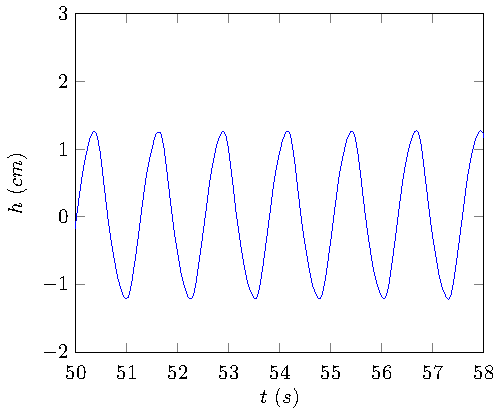
\includegraphics{WG1.pdf}} & & \resizebox{5cm}{!}{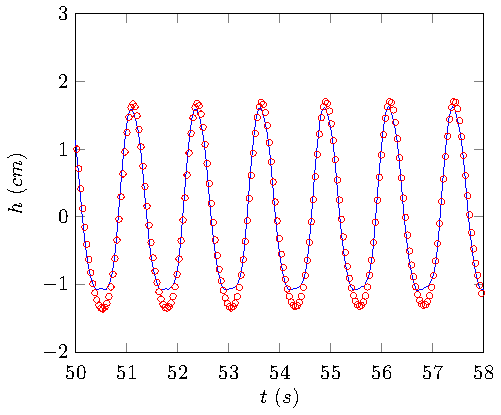
\includegraphics{WG2Serre.pdf}}  \\
		\hspace{5 mm} WG1 & & \hspace{5 mm}WG2 \\
		\resizebox{5cm}{!}{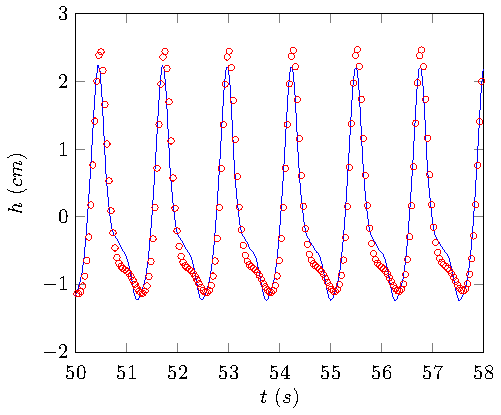
\includegraphics{WG3Serre.pdf}} && 
		\resizebox{5cm}{!}{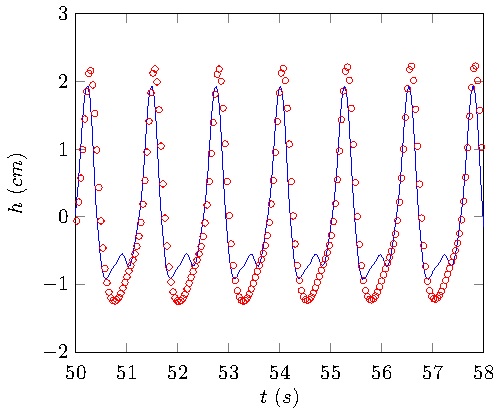
\includegraphics{WG4Serre.pdf}}  \\
		\hspace{5 mm} WG3 & & \hspace{5 mm} WG4 \\
		
		
	\end{tabular}
	\caption{Wave height readings from various wave gauges from the experiment of \cite{Beji-Battjes-1994} ({\color{blue} \solidrule}) compared to a simulation of the experiment using the Serre equations ({\color{red} $\circ$}).}
	\label{fig:WGSerre}
\end{figure}

\begin{figure}
	\centering
	\begin{tabular}{ccc}
		\resizebox{5cm}{!}{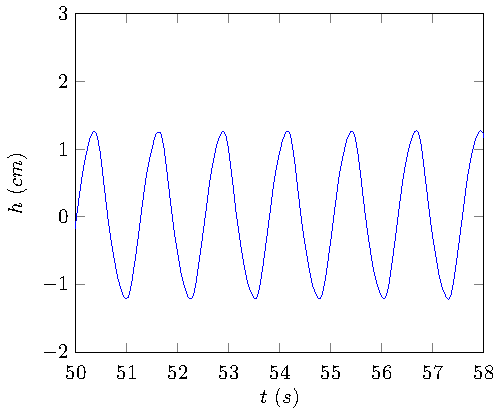
\includegraphics{WG1.pdf}} & & \resizebox{5cm}{!}{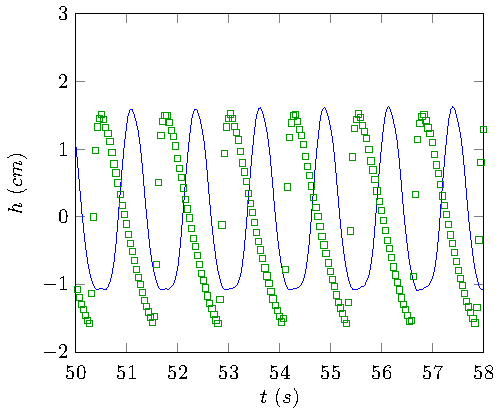
\includegraphics{WG2SWW.pdf}}  \\
		\hspace{5 mm} WG1 & & \hspace{5 mm}WG2 \\
		\resizebox{5cm}{!}{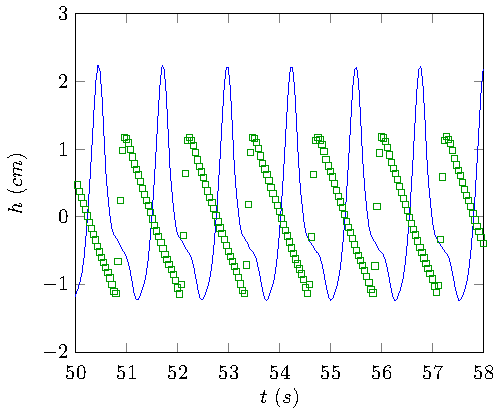
\includegraphics{WG3SWW.pdf}} && 
		\resizebox{5cm}{!}{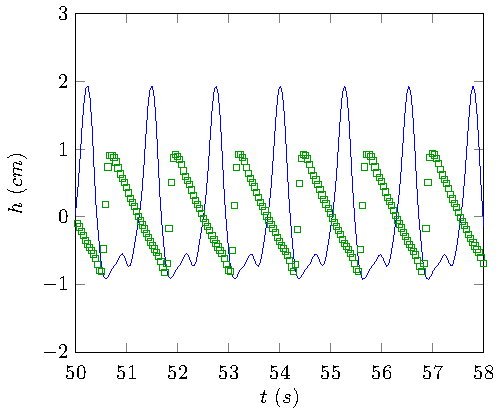
\includegraphics{WG4SWW.pdf}}  \\
		\hspace{5 mm} WG3 & & \hspace{5 mm} WG4 \\
		
		
	\end{tabular}
	\caption{Wave height readings from various wave gauges from the experiment of \cite{Beji-Battjes-1994} ({\color{blue} \solidrule}) compared to a simulation of the experiment using the shallow water wave equations ({\color{green!60!black} $\square$}).}
	\label{fig:WGSWW}
\end{figure}



\begin{figure}
	\centering
	\begin{tabular}{ccc}
		\resizebox{5cm}{!}{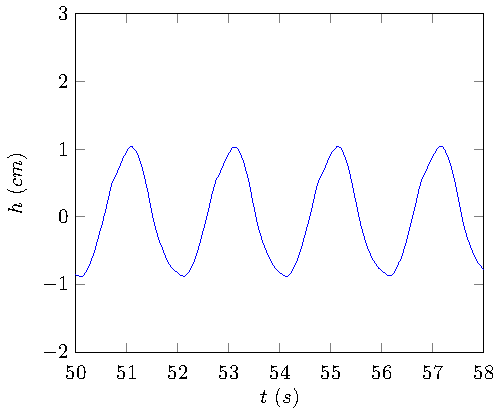
\includegraphics{SLWG1.pdf}} & & \resizebox{5cm}{!}{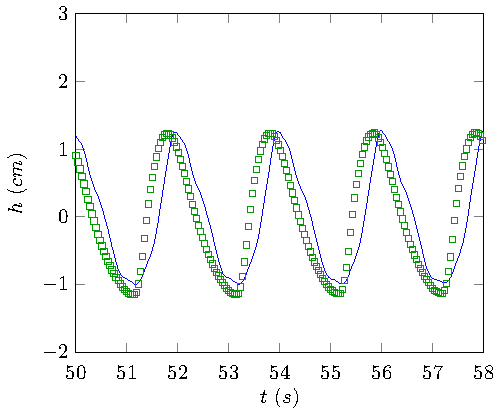
\includegraphics{SLWG2SWWE.pdf}}  \\
		\hspace{5 mm} WG1 & & \hspace{5 mm}WG2 \\
		\resizebox{5cm}{!}{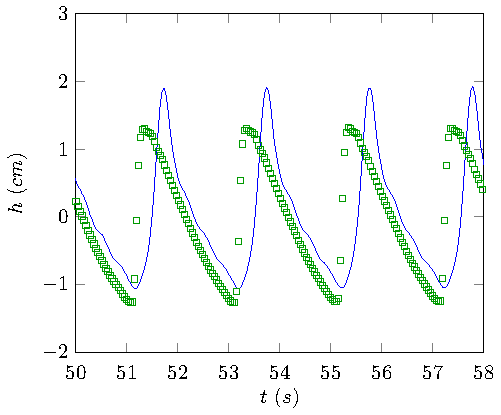
\includegraphics{SLWG3SWWE.pdf}} && 
		\resizebox{5cm}{!}{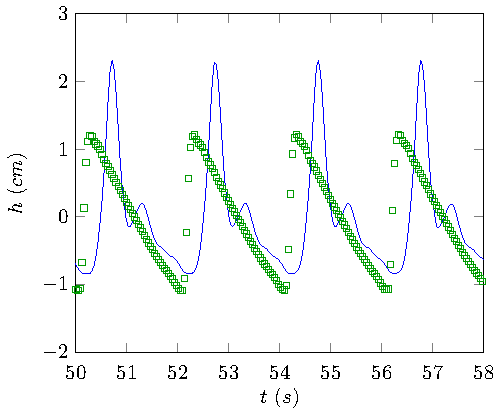
\includegraphics{SLWG4SWWE.pdf}}  \\
		\hspace{5 mm} WG3 & & \hspace{5 mm} WG4 \\
		
		
	\end{tabular}
	\caption{Wave height readings from various wave gauges from longer wavelength the experiment of \cite{Beji-Battjes-1994} ({\color{blue} \solidrule}) compared to a simulation of the experiment using the shallow water wave equations ({\color{green!60!black} $\square$}).}
	\label{fig:SLWGSWW}
\end{figure}



	
%--------------------------------------------------------------------------------
\section{Propagation of a Soliton over a Slope.}
\label{Soliton up a Slope}
%--------------------------------------------------------------------------------
The numerical results for the propagation of periodic waves over a submerged bar demonstrated large differences between the Serre and shallow water wave equations. These differences are pronounced due to the fact that the experimental set-up had waves with a wavelength that is comparable to the water depth, which is not appropriate for the shallow water wave equations. To rectify this another numerical experiment was performed simulating the propagation of a long wavelength, small amplitude wave over a uniformly sloping beach.  

In this simulation the initial conditions are the soliton of the Serre equations from \cite{El-etal-2006} with an amplitude of $0.01m$ on top of quiescent water $1m$ deep. The water depth is kept at a fixed $1m$ throughout the scenario. The bed profile is defined in the following way; $(x,b) = [$($-100$m,$0$m), ($100$m,$0$m), ($149.5$m,$0.99$m), ($250$m,$0.99$m)$]$. This scenario simulates the propagation of a relatively small amplitude wave over large horizontal distances, over a relatively shallow slope much like a tsunami propagating up a beach. The initial conditions and the numerical solutions for both the Serre equations and the shallow water wave equations are plotted in Figure \ref{fig:allstructs}.

It can be seen that the behaviour of the numerical solutions of the Serre equations and the shallow water wave equations are very similar when the wavelength is large compared to the depth. There is very little wave deformation for both equations after $t=20s$. For the Serre equations the soliton travels without deformation due to a balance between non-linearity and dispersion. For the shallow water wave equations the soliton travels with little deformation because the effect of non-linearity is small, as the wave amplitude is small. As the soliton progresses up the slope there is also very little difference between the numerical solutions throughout the shoaling process as can be seen at $t=40s$. It is only when the bed becomes flat after the slope that differences begin to arise although both numerical solutions are quite similar at $t=60s$ and at $100s$. The main difference between the Serre equations and the shallow water wave equations is the emergence of undulations trailing the bore that has formed. These oscillations have been observed in well validated numerical solutions of the Serre equations such as those of \cite{Mitsotakis-etal-2014} and even the Euler equations as shown by \cite{Mitsotakis-etal-2017}. These undulations oscillate around the bore of the shallow water wave equations, significantly increasing its maximum amplitude. It was demonstrated by \cite{Pitt-2017} that undular bores of the Serre equations travel slightly quicker than the bores of the shallow water wave equations. This suggests that the shallow water wave equations will slightly underestimate the arrival time as well as the maximum amplitude of an advancing wave.

\begin{figure}
	\centering
	\begin{tabular}{ccc}
		\resizebox{5cm}{!}{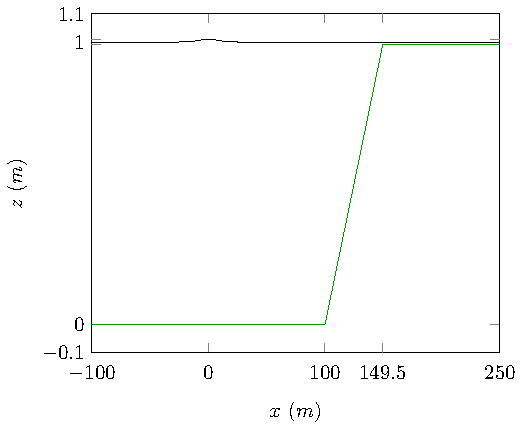
\includegraphics{solitonslopeSerre1.pdf}} & & \resizebox{5cm}{!}{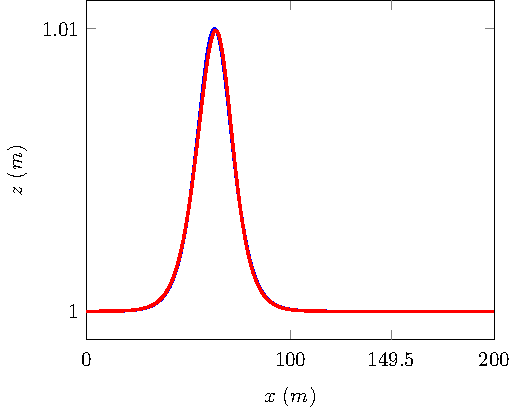
\includegraphics{solitonslopeSerre2.pdf}}  \\
		\hspace{5 mm} $t= 0s$ & & \hspace{5 mm}$t= 20s$ \\
		\resizebox{5cm}{!}{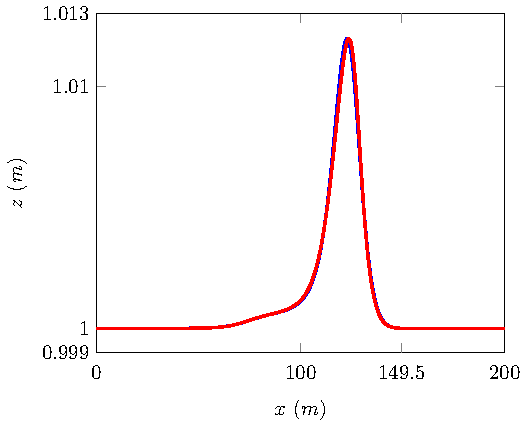
\includegraphics{solitonslopeSerre3.pdf}} && 
		\resizebox{5cm}{!}{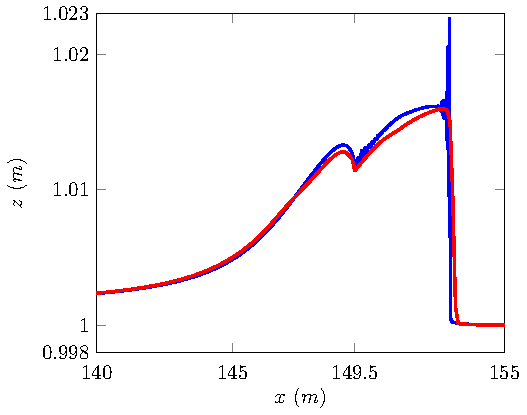
\includegraphics{solitonslopeSerre4.pdf}}  \\
		\hspace{5 mm} $t= 40s$ & & \hspace{5 mm} $t= 60s$ \\
		\resizebox{5cm}{!}{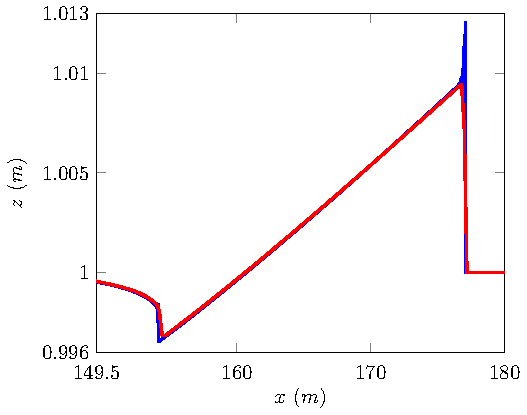
\includegraphics{solitonslopeSerre5.pdf}} && 
		\resizebox{5cm}{!}{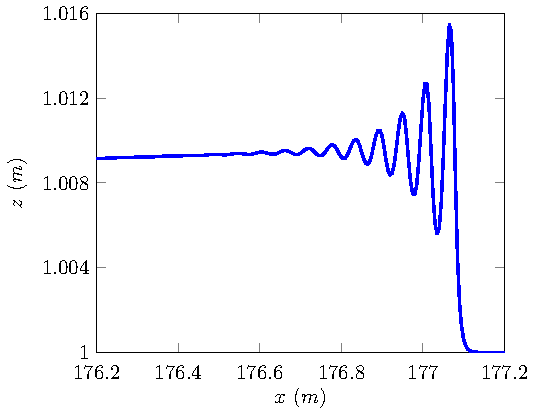
\includegraphics{SerreBore.pdf}}  \\
		\hspace{5 mm} $t= 100s$ & & \hspace{5 mm} front of bore at $t= 100s$ \\
		
		
	\end{tabular}
	\caption{The water profile from the numerical solution for the Serre equations ({\color{blue} \solidrule}) and the shallow water wave equations ({\color{red} \solidrule}) for the soliton travelling over a slope, at different times. The initial conditions for both numerical models are also presented in terms of stage ({\color{black} \solidrule}) and bed profile ({\color{green!60!black} \solidrule}).}
	\label{fig:allstructs}
\end{figure}


%--------------------------------------------------------------------------------
\section{Conclusions}
\label{Conclusions}
Well-validated numerical methods for the Serre and shallow water wave equations  were used to investigate the effect of dispersion on shoaling waves. It was demonstrated that when the wavelength is far larger than the water depth, dispersion is negligible during shoaling. However, dispersion is significant during the propagation of these shoaled waves over relatively thin water. As the wavelength becomes smaller compared to the water depth dispersion plays a larger role in the shoaling and the propagation of waves over flat bathymetry. These results demonstrate the need for the Serre equations to accurately capture fluid behaviour in the near shore where waves are shorter and the adequacy of the shallow water wave equations for modelling long waves. 


%--------------------------------------------------------------------------------	
\bibliographystyle{chicago} %use chicago style of referencing.
\bibliography{DamBreak}
\end{document}
